\documentclass{article}
\usepackage[T1]{fontenc}
\usepackage{microtype,graphicx,booktabs}
\usepackage{hyperref}
\usepackage{xurl}
\usepackage[preprint]{icml2026}
\usepackage{amsmath,amssymb,amsthm}
\newtheorem{theorem}{Theorem}
\DeclareMathOperator{\diag}{diag}
\DeclareMathOperator{\softmax}{softmax}
\newcommand{\norm}[1]{\lVert #1\rVert_2}
\newcommand{\tf}{f_\phi}
\newcommand{\pct}[1]{#1\%}
\icmltitlerunning{Information Sensitivity in Transformer Inverse Learning}
\begin{document}
\twocolumn[
\icmltitle{Stability and Information Sensitivity in Transformer In-Context Inverse Learning}
\begin{icmlauthorlist}
\icmlauthor{Fei Zhang}{course}
\end{icmlauthorlist}
\icmlaffiliation{course}{University of Waterloo}
\icmlcorrespondingauthor{Fei Zhang}{f243zhan@uwaterloo.ca}
\icmlkeywords{Transformer stability, in-context learning, inverse optimization}
\vskip 0.3in
]
\printAffiliationsAndNotice{}

\begin{abstract}
We examine how a frozen Transformer balances replacement stability
with responsiveness to informative observations. For the implemented
mean-pooled encoder we prove a \(C/m\) replacement bound, including
residual connections and LayerNorm. We construct two individually
identifying economic-dispatch contexts differing in one price, giving
a recovery error floor for any estimator obeying that bound. Across
three seeds, a matched price intervention produces a \(14.1\times\)
larger Transformer response under high leverage, while its response
on the identifying pair recovers only \pct{47.4} of the true parameter
difference at \(m=64\). Stability and accurate recovery depend on how
the context distributes its identifying information.
\end{abstract}

\section{Question and Contribution}
\citet{li} relate Transformer in-context learning to algorithmic
stability and generalization. A context can nevertheless concentrate
an entire parameter direction in one observation. We ask whether a
stable Transformer responds sufficiently to that observation for
accurate task recovery. Economic dispatch supplies a tractable setting
where the information in optimal decisions and prices can be checked.

\textbf{Positioning.} We rigorously examine a stability claim for our
architecture and stress-test its recovery implications. The
mean-pooled proof adapts the bounded-attention argument to the
implemented residual and normalization maps. The lower bound uses
the general triangle inequality and is related to stability-constrained
estimation \citep{clb}. Our concrete additions are the valid dispatch
construction, architecture audit and matched behavioral tests.
Inverse optimization provides the observation model
\citep{keshavarz,liang}. Frozen, context-dependent parameter estimation
also connects to investigations of regression algorithms in ICL
\citep{akyurek}.

\section{Setup}
At demand \(d\), two unit-capacity generators minimize
\begin{equation}
\min_{\substack{x_1+x_2=d\\0\le x_i\le1}}
\sum_{i=1}^2(a_ix_i+b_ix_i^2/2).
\label{eq:dispatch}
\end{equation}
The task parameter is \(\theta=(a_1,b_1,a_2,b_2)\), with
\(a_i\in[1,1.65]\) and \(b_i\in[0.8,2]\). Each record contains
\((d,x_1,x_2,\lambda,s_1,s_2)\), including the clearing price and
bound statuses. Positive \(b_i\) give unique dispatch. For an interior
unit, KKT stationarity gives \(\lambda=a_i+b_ix_i\). At the lower
bound marginal cost is at least the price, and at the upper bound it
is at most the price.

\textbf{Estimator.} Four scaled continuous features and two one-hot
statuses form ten inputs per record. Two 64-wide full-attention
layers use four heads, post-residual LayerNorm and 128-wide ReLU
feedforward blocks. Mean pooling and a sigmoid affine-box head
predict the four costs. Dropout is zero and positional encodings
are absent. Supervised source-task training minimizes span-scaled
parameter MSE, with frozen weights on new tasks. This is
\emph{context-conditioned supervised amortized inverse estimation}.
Li et al.'s model predicts a designated query response from a
sequence of examples \citep{li}; our readout estimates the task itself.

\section{Stability and Recovery}
\begin{theorem}[Encoder replacement stability]
\label{thm:upper}
Fix finite weights and depth for the encoder above, with positive
LayerNorm epsilon and bounded record features. In exact arithmetic,
there is a finite \(C\), independent of \(m\), such that any
length-\(m\) contexts differing in one record obey
\(\norm{\tf(S)-\tf(S')}\le C/m\).
\end{theorem}
\textit{Proof outline.} Write \(e_i=\norm{h_i-h_i'}\) and
\(\bar e=m^{-1}\sum_i e_i\). Initially \(\bar e=O(1/m)\).
Bounded attention scores imply probabilities at most \(e^{2B}/m\).
Integrating the softmax Jacobian controls query and key changes,
so each head multiplies \(\bar e\) by a fixed constant. Finite
residual, feedforward and LayerNorm Lipschitz factors preserve the
rate. Mean pooling and the readout give the claim. Appendix
\ref{app:encoder} supplies the full proof. This covers our set readout;
Li et al.'s Theorem 3.2 covers a query token under their normalization
assumptions \citep{li}.

\begin{theorem}[Necessary response]
\label{thm:lower}
Suppose \(S,S'\) differ in one record and have true parameters
\(\theta,\theta'\) at distance \(D\). If an estimator has Euclidean
error at most \(\epsilon\) on both, its predictions differ by at
least \(D-2\epsilon\). If their change is at most \(C/m\), then
\(\epsilon\ge(D-C/m)_+/2\).
\end{theorem}
\begin{proof}
The triangle inequality gives
\[
D\le\norm{\theta-f(S)}+\norm{f(S)-f(S')}
     +\norm{f(S')-\theta'}.
\]
Substitute both error bounds and rearrange.
\end{proof}

\textbf{Valid construction.} Task A uses \((a_i,b_i)=(1.6,1)\)
and task B uses \((1.2,1.8)\) for both generators. Symmetry gives
\(x_i=d/2\). At \(d=1\), both give the record
\((x_1,x_2,\lambda)=(0.5,0.5,2.1)\).
At \(d=1.6\), dispatch is \((0.8,0.8)\) in both, and prices are
2.40 and 2.64. Repeat the common record \(m-1\) times and append
the distinguishing record. Each context uniquely identifies both
affine costs from two distinct interior outputs, while the targets
are separated by \(D=\sqrt{1.6}\).

For a fixed encoder, this family forces a limiting worst-case error
floor \(D/2\). It does not give an average error floor under uniform
random demands: the exact repetitions are a deliberate stress case.
The weight-derived \(C\) is very loose, with uncapped checkpoint
\(\log_{10}C\) between 616.5 and 708.9. Thus the rate alone supplies
no calibrated prediction for the tested \(m\).

\section{Experiments}
All results use seeds 886, 1729 and 2027 with task-disjoint splits,
96 validation tasks and 128 unseen test tasks per seed. D and G
train on 1,536 source tasks for 14 epochs using AdamW, batch size
32, and validation checkpoint selection. Ordinary demands are
uniform on \([0,2]\). We measure relative recovery error
\(E=\norm{\tf(S)-\theta}/\norm{\theta}\) and sampled prediction
change \(\Delta=\norm{\tf(S)-\tf(S')}\). Means weight seeds equally.
All predictions here precede any KKT correction.

\textbf{Architecture (D).} Replace one record by another valid
observation from the \emph{same} task, four times per task at each
\(m\in\{4,8,16,32,64\}\). The original Transformer has the lowest
mean change and error at every length among itself, a Transformer
with Q/K/V/output norm caps of 0.85, and DeepSets
\citep{deepsets}. At \(m=64\), their respective
\((\Delta,E)\) are \((0.00213,\pct{2.65})\),
\((0.00510,\pct{3.95})\), and \((0.00760,\pct{10.28})\).
This finite-budget comparison does not order their worst-case
constants. Full curves appear in Appendix \ref{app:details}.

\textbf{Transfer (E).} At \(m=32\), equal-pass error falls from
\pct{13.48} to \pct{2.72} as source tasks increase from 128 to 1,536,
but updates also rise from 56 to 672. With 448 updates, errors
range nonmonotonically from \pct{3.20} to \pct{3.56}. The supporting
task-risk bound in Appendix \ref{app:transfer} uses IID tasks and a
fixed hypothesis class. This sweep does not establish a monotonic
task-count effect at fixed compute.

\textbf{Conditioning (F).} For each task select 16 valid records
with different information structure. Define
\(H_i=m^{-1}\sum_{t:\,s_{it}=\mathrm{int}}u_{it}u_{it}^{\top}\),
\(u_{it}=(1,x_{it})^\top\), and
\(\mu=\min_i\lambda_{\min}(H_i)\). Table \ref{tab:f}
shows that near-redundant contexts uniquely identify costs but
yield poor learned recovery. Interior regimes share mean demand;
their spreads differ. Bound-heavy contexts also shift demand.

\begin{table}[t]
\caption{F at \(m=16\). Error is mean \(\pm\) seed SD, in percent.
The first three regimes uniquely identify costs.}
\label{tab:f}
\centering
\begin{tabular}{lrr}\toprule
Context&$\mu$&Error (\%)\\
\midrule
Well-conditioned & $0.03257$ & $2.90\pm0.30$ \\
Nearly redundant & $3.72\times10^{-6}$ & $13.65\pm0.57$ \\
Mixed & $0.02429$ & $3.72\pm0.08$ \\
Boundary-heavy & $0$ & $17.64\pm0.72$ \\
\bottomrule\end{tabular}

\end{table}

\begin{figure*}[t]
\centering
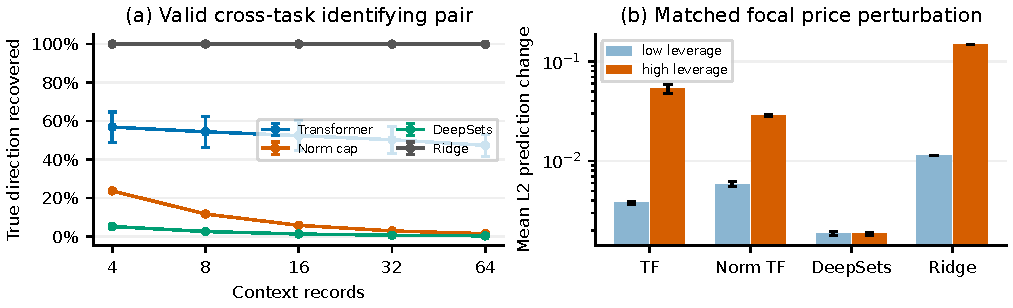
\includegraphics[width=\textwidth]{results/course_report/information_response.pdf}
\caption{G. (a) Signed projection of prediction change on the true
parameter difference, divided by its squared norm, on the valid
cross-task pair. (b) One focal price changes from \(\lambda-0.01\)
to \(\lambda+0.01\) in matched background designs. Error bars are
one SD across three seed means. These two protocols probe different
requirements for response.}
\label{fig:g}
\end{figure*}

\textbf{Matched interventions (G).} Holding the focal observation
and edit fixed, we cross a clustered or spread background on the
same task. Mean focal hat leverage is 0.999 versus 0.133.
A price edit of 0.02 produces mean changes 0.0535 versus 0.00379
for the original Transformer (\(14.1\times\)), and 0.1488 versus
0.01137 for ridge (\(13.1\times\)); see Figure \ref{fig:g}.
The Transformer shares a conditioning-dependent response with
ridge but has a smaller absolute response. The within-task clean
edit keeps the true costs fixed, while the identifying construction
changes the task. On the latter at \(m=64\), Transformer directional
recovery is \pct{47.4}, with larger endpoint error 0.432 in Euclidean
units; ridge recovers \pct{99.9}. A statistics MLP and DeepSets
recover less than \pct{0.4}. Their lower response accompanies
poorer recovery on this pair.

\section{Discussion and Conclusion}
The information concentrated in the identifying record forces a
response of at least \(D-2\epsilon\) from an accurate estimator.
When identifying records number \(k\), a bounded-input replacement
path gives an upper bound \(kC/m\) by telescoping. For the completed
192-pair replication at \(m=64\), moving from one to eight identifying
records raises uncapped directional response from \pct{50.0} to
\pct{54.7}. The largest step on that specified path falls from
0.301 to 0.074, averaged over pairs and seeds. Both valid endpoints
identify their respective costs. Intermediate mixtures of their
prices need not correspond to a single noiseless task.

Table \ref{tab:e-main} makes the transfer confound explicit.
The fixed-length follow-up allocates 384 updates, batch size 32,
and 16 records per training context, for 196,608 record
presentations. It fixes initialization, demand draws and the
final-checkpoint time across source sets. Target errors at \(m=32\)
are \pct{3.48}, \pct{3.25}, and \pct{3.54} for \(T=128,512,1536\).
The source-task-count trend remains nonmonotonic.

\begin{table}[h]
\caption{E target errors at \(m=32\), in percent. Equal-pass runs
use the listed updates; equal-step runs use 448.}
\label{tab:e-main}
\centering
\begin{tabular}{rrrr}\toprule
$T$&Updates&Equal pass&Equal step\\
\midrule
128 & 56 & 13.48 & 3.29 \\
256 & 112 & 10.45 & 3.47 \\
512 & 224 & 7.46 & 3.54 \\
1,024 & 448 & 3.20 & 3.20 \\
1,536 & 672 & 2.72 & 3.56 \\
\bottomrule\end{tabular}

\end{table}

For a clean same-task replacement, both contexts retain the same
true costs. The original Transformer changes by 0.0314 under the
high-leverage edit and 0.00197 under the low-leverage edit.
The near-OLS ridge fit changes by 0.0000720 and 0.000000591.
In the price intervention the design stays fixed while its
right-hand side changes. Sharing ridge's relative sensitivity to
background conditioning therefore falls short of reproducing its
input-output behavior across these protocols.

The matched backgrounds fix the focal record's feature location
and displacement. Their output spread and conditioning vary by
construction. A broader context also changes the input distribution
relative to training. The Gram eigenvalues describe constraints
in the observations, while neural recovery depends additionally
on the source distribution and optimization. Partial identification
in the bound-heavy regime leaves a mean admissible diameter 1.056.
Even an exactly consistent estimator must select among compatible
costs there using its prior.

This study connects an architecture-specific stability bound to a
general recovery constraint through a valid optimization example.
Matched interventions show that the learned response depends on
information in the background, yet can remain insufficient for
accurate recovery. The construction uses repeated demands and the
experiments use a small, mostly noiseless system and three seeds.
Distribution shifts and loose norm constants limit extrapolation.
Input-output interventions leave the internal attention algorithm
unresolved. The defensible conclusion is that a stability guarantee
must be assessed together with the identifying information and
recovery objective.

\clearpage
\bibliography{COURSE_PROJECT_REFERENCES}
\bibliographystyle{icml2026}
\clearpage
\appendix
\onecolumn

\section{Proof of Theorem~\ref{thm:upper}}
\label{app:encoder}
For row states \(h_i,h_i'\) at one layer input write
\(e_i=\norm{h_i-h_i'}\) and \(\bar e=m^{-1}\sum_i e_i\).
All state norms have a common bound at each fixed layer, independent
of \(m\). The embedding maps bounded inputs to bounded states.
Attention returns a convex combination of bounded values in each
head. The subsequent finite affine maps, residuals, and rowwise
nonlinearities preserve boundedness. In particular, centering and
normalizing a width-\(p\) row before its LayerNorm affine map gives
a vector of norm at most \(\sqrt p\).

For a head of dimension \(d_h\), let \(Q_0,K_0,V_0\) bound the norms
of its query, key and value vectors, including affine biases, and
write \(q,k,v\) for the operator norms of the corresponding linear
maps. Its score in row \(i\), column \(j\), is
\(s_{ij}=q_i^\top k_j/\sqrt{d_h}\). For the two input matrices we have
\[
 |s_{ij}|,|s'_{ij}|\le B=Q_0K_0/\sqrt{d_h},
 \qquad |s_{ij}-s'_{ij}|\le
 (qK_0e_i+kQ_0e_j)/\sqrt{d_h}.
\]
The latter follows by adding and subtracting the inner product of
the new query with the old key. On the line segment between the two
score rows, every softmax entry is at most \(e^{2B}/m\), since the
numerator is at most \(e^B\) and the denominator at least \(me^{-B}\).
For \(p=\softmax(s)\), the \(j\)-th column of its Jacobian has absolute
sum \(2p_j(1-p_j)\le2p_j\). Integrating this Jacobian along the segment
gives
\[
 \lVert p_i-p_i'\rVert_1
 \le \frac{2e^{2B}}{\sqrt{d_h}}(qK_0 e_i+kQ_0\bar e).
\]
For the head output, changing weights with values fixed costs at
most \(V_0\lVert p_i-p_i'\rVert_1\). Changing values with weights fixed
costs at most \(ve^{2B}\bar e\). Averaging over rows bounds the mean
head difference by \(J_h\bar e\), where
\[
 J_h=e^{2B}\left(v+\frac{2V_0(qK_0+kQ_0)}{\sqrt{d_h}}\right).
\]
Concatenation bounds its mean difference by the sum of the individual
head bounds. Applying \(W_O\) and adding the input residual gives a
factor at most \(1+\|W_O\|\sum_hJ_h\). Here and below, matrix norms
are induced Euclidean operator norms.

To bound LayerNorm, write \(P\) for the orthogonal projection onto
mean-zero rows. The map before its learned affine part is
\(h\mapsto Ph/(\|Ph\|_2^2/p+\eta)^{1/2}\), with \(\eta>0\).
The derivative of \(z\mapsto z/(\|z\|_2^2/p+\eta)^{1/2}\)
has tangential eigenvalue \((\|z\|_2^2/p+\eta)^{-1/2}\) and radial
eigenvalue \(\eta(\|z\|_2^2/p+\eta)^{-3/2}\). Each is at most
\(1/\sqrt\eta\). Consequently a LayerNorm with learned gain \(\gamma\)
has Lipschitz constant at most \(\|\gamma\|_\infty/\sqrt\eta\).
The two affine feedforward maps and ReLU, with their residual,
contribute another factor at most \(1+\|W_2\|\|W_1\|\).
Each of the two LayerNorm maps and both residual blocks therefore
have a finite layer product. This covers the implemented post-residual
block, with actual attention scores scaled by \(1/\sqrt{16}\).

Initially just one row differs and its embedded difference is at most
\(2R_{\rm in}\|W_{\rm emb}\|\), where \(R_{\rm in}\) bounds the record
feature norm. Thus \(\bar e_0\le 2R_{\rm in}\|W_{\rm emb}\|/m\).
The finite product of layer factors propagates this bound. The difference
of mean-pooled vectors is at most the final \(\bar e\) by the triangle
inequality. The sigmoid affine-box readout multiplies the bound by at
most \(\|\diag(\mathrm{span})\|\|W_{\rm head}\|/4\). This proves the
claim. The box gives a separate trivial bound on all outputs. For the
three uncapped checkpoints the norm substitution gave
\(\log_{10} C\) between 616.5 and 708.9, so the box is tighter over
the measured lengths.

\section{Supporting task-level transfer bound}
\label{app:transfer}
Let \(m\) be fixed and \(L_\theta(f)\) be the conditional expectation
of span-normalized squared parameter error over contexts from task
\(\theta\). Both estimates and targets are in the coefficient box,
so \(L_\theta(f)\in[0,1]\). Take \(T\) independent source tasks from
a population \(P\), and a fixed hypothesis class independent of those
tasks. For a finite \(\varepsilon\)-cover of the induced task-risk
functions in sup norm with size \(N_\varepsilon\), with probability
at least \(1-\delta\) all predictors in that class satisfy
\[
 \left|\mathbb E_{\theta\sim P}L_\theta(f)
   -\frac{1}{T}\sum_{t=1}^T L_{\theta_t}(f)\right|
 \le 2\varepsilon+\sqrt{\frac{\log(2N_\varepsilon/\delta)}{2T}} .
\]
For each center Hoeffding's inequality gives a two-sided tail
\(2e^{-2Tu^2}\) at deviation \(u\). A union bound controls every
center, and approximation of the population and empirical risks
costs \(\varepsilon\) each. At fixed \(m\), a deterministic compact
weight set gives a finite cover via uniform continuity of the
network and its bounded loss on the bounded record domain.
This argument controls the source-to-population risk difference
for that class. The numerical size of the cover, optimization
quality, and transfer under a different task distribution require
other information. The assumption of independent source tasks and
fresh evaluation contexts matches the in-distribution target
comparison in E. The bound makes no empirical rate prediction for
the optimization-budget sweep.


\section{Experimental Details and Additional Results}
\label{app:details}
\subsection{Architecture and Replacement Protocol}
The ten record features are $(d/2,x_1,x_2,\lambda/3.65)$ and two
three-way one-hot statuses. Width is 64, head dimension is 16,
feedforward width is 128, and LayerNorm epsilon is $10^{-5}$.
The original Transformer and norm-controlled version each have 67,908
trainable parameters; DeepSets has 63,396. AdamW uses learning rate
0.001 and its PyTorch default weight decay. Source coefficients are
sampled independently and uniformly within the stated box. The validation
score averages relative parameter error across the five context lengths.
The encoder operates on sets, and shuffling in F changed predictions
by $1.20\times10^{-7}$ on average, consistent with numerical evaluation
of its permutation-invariant construction.

\begin{table}[h]
\centering
\begin{tabular}{r rrr rrr}
\toprule
&\multicolumn{3}{c}{Mean prediction change}&\multicolumn{3}{c}{Recovery error (\%)}\\
\cmidrule(lr){2-4}\cmidrule(lr){5-7}
$m$&Transformer&Norm cap&DeepSets&Transformer&Norm cap&DeepSets\\
\midrule
4 & 0.07750 & 0.11445 & 0.11455 & 5.20 & 7.03 & 13.06 \\
8 & 0.02852 & 0.05117 & 0.06152 & 3.50 & 5.31 & 11.75 \\
16 & 0.01077 & 0.02273 & 0.02909 & 2.92 & 4.53 & 11.11 \\
32 & 0.00461 & 0.01062 & 0.01542 & 2.71 & 4.14 & 10.60 \\
64 & 0.00213 & 0.00510 & 0.00760 & 2.65 & 3.95 & 10.28 \\
\bottomrule\end{tabular}

\caption{D, means over three seeds. A valid same-task replacement is
generated independently for each trial. Context lengths use nested
uniform-demand contexts within each task.}
\label{tab:d}
\end{table}

\subsection{Transfer Risk and Budgets}
Source-task population-risk estimates average two fresh uniform contexts
per training task. Transfer estimates use two fresh contexts per unseen
test task, with identical target contexts across task-count comparisons.
Risk is the mean squared coefficient error divided coordinatewise by
the coefficient span. It is a different metric from relative Euclidean
parameter error. In the equal-step study at $T=128$ and $T=1536$,
the mean transfer risks at $m=32$ are 0.002686 and 0.003218.
Their transfer-minus-source gaps are 0.000517 and 0.000006. A smaller
gap can coexist with higher absolute target risk.

\begin{table}[h]
\centering
\begin{tabular}{r rrr}\toprule
Source tasks&Equal-pass updates&Equal-pass error (\%)&Equal-step error (\%)\\
\midrule
128 & 56 & 13.48 & 3.29 \\
256 & 112 & 10.45 & 3.47 \\
512 & 224 & 7.46 & 3.54 \\
1,024 & 448 & 3.20 & 3.20 \\
1,536 & 672 & 2.72 & 3.56 \\
\bottomrule\end{tabular}

\caption{E, unseen-task mean relative error at $m=32$.
Equal-step runs allocate 448 updates. All use batch size 32.
Validation selects a checkpoint within the allocated budget.}
\label{tab:e}
\end{table}

The fixed-length follow-up uses 384 updates with batches of 32 and
16 records, for exactly 196,608 record presentations per model. It
holds training demand draws, initialization and final-checkpoint time
fixed across nested source subsets. At evaluation length 32, the
errors are 3.48\%, 3.25\%, and 3.54\% for 128, 512, and 1,536
source tasks. Smaller sets expose the learner to the same tasks more
often. The task-count trend remains nonmonotonic.

\subsection{Information and Response Controls}
F builds an interior pool from 2,047 evenly spaced demands and selects
broad or tightly clustered outputs centered at the same demand.
The average within-context demand standard deviations are 0.450 and
0.00493. Mixed contexts contain eight interior and eight boundary
records; boundary-heavy contexts retain one fixed bound status.
The mean Wasserstein distance to the well-conditioned demand
distribution is 0.386, 0.444, and 0.889 for near-redundant, mixed,
and boundary-heavy contexts. Their information diagnostics summarize
both status and output spread.

\begin{table}[h]
\centering
\begin{tabular}{lrrr}\toprule
Context&$\mu$&Diameter&$E$ (\%)\\
\midrule
Well-conditioned & $0.03257$ & 0.000 & $2.90\pm0.30$ \\
Nearly redundant & $3.72\times10^{-6}$ & 0.000 & $13.65\pm0.57$ \\
Mixed & $0.02429$ & 0.000 & $3.72\pm0.08$ \\
Boundary-heavy & $0$ & 1.056 & $17.64\pm0.72$ \\
\bottomrule\end{tabular}

\caption{F, 16-record contexts on matched tasks. The Gram diagnostic
is the smallest interior-Gram eigenvalue across generators, normalized
by total context length. Error shows mean $\pm$ seed SD.}
\label{tab:f}
\end{table}

G supplies an additional control by fixing the focal record, edit and
direction across two backgrounds on the same task. Left- and right-side
focal locations are both tested. The maximal per-unit Gram condition
numbers average 772 under the clustered background and 58.9 under
the spread background. In the price intervention the raw feature
displacement is 0.00548 for both. Prices are measured as
$\lambda-\eta$ and $\lambda+\eta$, with $\eta=0.01$ or $0.04$.
The perturbation is a measurement edit; the clean dispatch endpoints
remain exact forward solutions.

The ridge baseline solves
$(H_i+\rho I)^{-1}(g_i+\rho\theta_{0i})$ using interior
$H_i=m^{-1}\sum_t u_{it}u_{it}^\top$ and
$g_i=m^{-1}\sum_tu_{it}\lambda_t$, with the sums restricted to
interior records. Its prior is the source-task mean. Validation on
uniform contexts selects $\rho=10^{-6}$ for all seeds, the smallest
tested value. The statistics MLP receives the unique entries of
$H_i$ and scaled $g_i$ for both units as ten features. It uses two
96-wide hidden layers and the same supervised training schedule.
The signed directional response in Figure~\ref{fig:g} is
\[
r=\frac{\langle f(S')-f(S),\theta'-\theta\rangle}
         {\|\theta'-\theta\|_2^2}.
\]
A value of one indicates complete response along the target difference.
Perpendicular prediction errors can remain.

\subsection{Completed Follow-up Studies}
The 192-pair dispatch replication holds the target separation at 0.6
and focal price gap at 0.09. At $m=64$, increasing identifying records
from one to eight raises uncapped directional response from 50.0\%
to 54.7\%. The largest step on the specified replacement path drops
from 0.301 to 0.074, averaged over pairs and seeds. Intermediate price
mixtures on this path need not correspond to one noiseless task;
the two evaluated recovery endpoints are valid.

The cap sweep tests 0.50, 0.85, 1.25 and 2.00 with the same training
budget. At $m=64$, their ordinary relative errors are 5.53\%, 3.96\%,
3.36\%, and 2.59\%. Their responses to the single identifying
record recover 3.18\%, 26.1\%, 23.7\%, and 39.5\% along the
target difference. Ordinary and cross-task response comparisons
therefore answer distinct empirical questions.

With independent Gaussian noise on all context prices at
standard deviation 0.04, near-redundant-context errors are 13.67\%
for the frozen Transformer and 15.28\% for box-clipped ridge tuned
on noisy validation tasks. Well-conditioned errors are 3.87\% and
2.39\%, and boundary-heavy errors are 17.41\% and 15.50\%.
Dispatch and statuses remain exact, fixing the design matrices.

\section{Reproducibility}
The accompanying archive contains the Python source, tests, experiment
configurations, saved CSVs, checkpoints and report assets. Synthetic
data are generated by the analytical dispatch solver; no external
dataset or account is required. The source/validation/test split is
by cost task. The \texttt{REPRODUCIBILITY.md} file gives setup,
test, rerun and report-build commands. \texttt{scripts/build\_report\_assets.py}
regenerates Tables~\ref{tab:d}--\ref{tab:f} and the main figure directly
from the saved D--G summaries. A SHA-256 manifest records the packaged
file bytes. Floating-point results may depend on package versions and
hardware. The archive includes the measured versions and the saved
configuration for each study.
\end{document}
